Let $k(x)$ and $p(x)$ be two positive-valued continuous functions on $[0,1]$.  
\begin{enumerate}
\item Define
\[ V = C^2_D[0,1] = \Big\{ u\in C^2[0,1]: u(0) = u(1) = 0 \Big\}.\]
 Derive the weak form of the differential equation
\[ -{d\over dx} \Big(k(x) {du \over dx}\Big) + p(x) u = f(x), 
    \quad 0 < x< 1,\]
subject to the boundary conditions
\[  u(0) = u(1) = 0;\]
that is, transform this differential equation into a problem of the form:
\[\mbox{Find $u \in V$ such that $a(u,v) = (f,v)$ for all $v\in V$},\]
where $(\cdot,\cdot)$ denotes the usual inner product
$(f, g) = \int_0^1 f(x) g(x)\, dx$,
and $a(\cdot, \cdot)$ is some bilinear form that you should specify.  Verify that $a(u,v)$ is still an inner product.  
\item Let $p(x) = 1$, $k(x) = \epsilon$, and let the source function $f(x) = 1$.  Construct the finite element system $A\alpha = b$, where
\[
A_{ij} = a(\phi_j,\phi_i), \quad b_i = \int_0^1 f(x)\phi_i(x)
\]
using the approximation space $V_N$ given by the piecewise linear
\emph{hat functions}:
for $n\ge 1$,  $h = 1/(N+1)$,  and $x_k = kh$ for $k = 0, \ldots, N+1$,
we have 
\[ \phi_k(x) = \left\{ \begin{array}{ll}
           (x-x_{k-1})/h, & x\in [x_{k-1}, x_k);\\
           (x_{k+1}-x)/h, & x\in [x_k, x_{k+1});\\
            0,             & \mbox{otherwise}.
          \end{array}\right. \]
          
\emph{Hint: for this specific choice of $p(x),k(x)$, it may be easier to show that you can express
\[
A = \epsilon K + M, \quad K_{ij} = \int_0^1 \frac{\partial \phi_j}{\partial x}\frac{\partial \phi_i}{\partial x}
\]
where the form of $M$ is specified in Homework 6, 4(d).}
\item This specific equation corresponds to the simplest steady-state \emph{reaction-diffusion} equation, where $u(x)$ is the concentration of some solvent, and the choices of $p(x)$ model local chemical reactions that may occur due to that solvent (multiple chemicals interacting may be modeled using \emph{systems} of reaction-diffusion equations).  

Solve the above system with $N = 32$ and $\epsilon = .1, .25, 1$.  What do you observe about the solution as $\epsilon$ becomes smaller?
\item Let the space $V$ now be defined as
\[ V = \Big\{ u\in C^2[0,1]: u(0) = {du\over dx}(1) = 0 \Big\}.\]
Derive the weak form of the differential equation
\[ -{d\over dx} \Big(k(x) {du \over dx}\Big) + p(x) u = f(x), 
    \quad 0 < x< 1,\]
subject to the boundary conditions
\[  u(0) = {du\over dx}(1) = 0;\]
that is, transform this differential equation into a problem of the form:
\[\mbox{Find $u \in V$ such that $a(u,v) = (f,v)$ for all $v\in V$},\]
where $(\cdot,\cdot)$ denotes the usual inner product
$(f, g) = \int_0^1 f(x) g(x)\, dx$,
and $a(\cdot, \cdot)$ is some bilinear form that you should specify.

\item Show that the form $a(u,v)$ from part~(d) is an inner product
      for $u, v \in V$.
\end{enumerate}
%%%%%%%%%%%%%%%%%%%%%%%%%%%%%%%%%%%%%%%%%%%%%%%%%%%%%%%%%%%%%%%%%%%%%%%%%%%%%%%%

\ifthenelse{\boolean{showsols}}{\begin{solution}
\begin{enumerate}
\item Multiply the differential equation with some function $v$
      from the space $V$ and integrate from $x=0$ to $x=1$ to obtain
     \[ \int_0^1 \bigg(-{d\over dx} \Big(k(x) {du \over dx}(x)\Big) v(x)
                      + p(x) u(x) v(x) \bigg)\,dx   
          = \int_0^1 f(x)v(x)\,dx.\]
      Break the integral on the left into pieces to obtain
     \[  \int_0^1 \bigg(-{d\over dx} \Big(k(x) {du \over dx}(x)\Big)\bigg) v(x)\,dx
       + \int_0^1 \bigg( p(x) u(x)\bigg) v(x)\,dx 
       = \int_0^1 f(x)v(x)\, dx.\]
     Integrate the first integral by parts to obtain
     \[ -\Big[ \kappa(x) {du \over dx}(x) v(x) \Big]_0^1 
        + \int_0^1 k(x) {du \over dx}(x) {dv\over dx}(x)\,dx
       + \int_0^1 \Big( p(x) u(x)\Big) v(x)\,dx 
       = \int_0^1 f(x)v(x)\, dx.\]
       The boundary terms vanish due to the fact that $v(0) = v(1) = 0$ if $v\in V= C^2_D[0,1]$.  
       We consolidate the integrals
     on the left to arrive at the weak problem:
      \[ \mbox{Find $u\in V$ such that}\quad
          a(u,v) = (f,v) \quad \mbox{for all $v\in V$},\]
     where 
     \[ a(u,v) = 
         \int_0^1 \Big( k(x) {du \over dx}(x) {dv\over dx}(x)
                       + p(x) u(x) v(x)\Big)\,dx.\]
       

To show that the form $a(u,v)$ in part~(a) is an inner product, 
      we must verify the three basic properties:
      \begin{itemize}
      \item \textbf{Symmetry} is apparent by inspection:
            \begin{eqnarray*}
               a(u,v) 
               &=& \int_0^1 \Big( k(x) {du \over dx}(x) {dv\over dx}(x)
                              + p(x) u(x) v(x)\Big)\,dx \\[0.5em]
               &=& \int_0^1 \Big( k(x) {dv \over dx}(x) {du\over dx}(x)
                              + p(x) u(x) v(x)\Big)\,dx
               \,=\, a(v,u).
           \end{eqnarray*}

      \item \textbf{Linearity} follows from the
            linearity of differentiation and integration:
            \begin{eqnarray*}
              a(\alpha u + \beta v, w)
               &=& \int_0^1 \Big( k(x) {d(\alpha u(x) + \beta v(x))\over dx}(x) {dw\over dx}(x)
                              + p(x) (\alpha u(x) + \beta v(x)) w(x)\Big)\,dx \\[0.5em]
               &=& \int_0^1 \Big( k(x) \Big(\alpha {du(x)\over dx} + \beta{dv(x)\over dx}\Big) {dw\over dx}(x)
                              + p(x) (\alpha u(x) + \beta v(x)) w(x)\Big)\,dx \\[0.5em]
               &=& \alpha \int_0^1 \Big( k(x) {du(x)\over dx} {dw\over dx}(x) + 
                                            p(x) u(x) w(x)\Big)\,dx \\[0.25em]
               && \ \ \ 
                   +\beta \int_0^1 \Big( k(x) {dv(x)\over dx} {dw\over dx}(x) + 
                                            p(x) v(x) w(x)\Big)\,dx  \\[0.5em]
               &=& \alpha @ a(u,w) + \beta @ a(v,w).
               \end{eqnarray*}
      \item \textbf{Positivity} requires that $a(u,u) \ge 0$ and $a(u,u) = 0$ only when $u=0$.
            Note that
               \begin{eqnarray*}
               a(u,u) &=& \int_0^1 \Big( k(x) {du \over dx}(x) {du\over dx}(x)
                              + p(x) u(x) u(x)\Big)\,dx \\[0.5em]
                      &=& \int_0^1 \Big( k(x) \Big({du \over dx}(x)\Big)^2 
                              + p(x) \big(u(x)\big)^2 \Big)\,dx.
               \end{eqnarray*}
            Since $k(x)$ and $p(x)$ are both positive for all $x\in[0,1]$, 
            each integrand is non-negative, and hence $a(u,u)\ge 0$.
            To have $a(u,u)=0$, we must have $u(x) = 0$ for all $x\in[0,1]$,
            and $du(x)/dx = 0$ for all $x\in[0,1]$, which is only possible
            if $u(x)=0$ for all $x\in[0,1]$, i.e., $u=0$.
      \end{itemize}
\item If $p(x) = 1$ and $k(x) = \epsilon$, our formulation reduces down to $a(u,v) = (f,v)$ where
\[
a(u,v) = \int_0^1 u(x) v(x) dx + \epsilon \int_0^1 \frac{\partial u}{\partial x}\frac{\partial v}{\partial x} dx.
\]
Then, if $A_{ij} = a(\phi_j,\phi_i)$, we have 
\[
A_{ij} = \int_0^1 \phi_j(x) \phi_i(x) dx + \epsilon \int_0^1 \frac{\partial \phi_j}{\partial x}\frac{\partial \phi_i}{\partial x} dx = M_{ij} + \epsilon K_{ij}
\]
where $M_{ij} = \int_0^1 \phi_j(x) \phi_i(x) dx$ is the Gram matrix for hat functions using the $L^2$ inner product.  The entries of $M$ and $K$ are known to be
\[
M_{ij} = \begin{cases}
M_{i,i} &= 2h/3\\
M_{i+1,i} &= h/6\\
M_{ij} &= 0, \quad |i - j| > 1
\end{cases}, \quad 
K_{ij} = \begin{cases}
K_{i,i} &= 2/h\\
K_{i+1,i} &= -1/h\\
K_{ij} &= 0, \quad |i - j| > 1
\end{cases}
\]
from class and from previous homeworks.  
\item The code to generate the figures for this problem are given below.  
\input reacdiff_code
\begin{center}
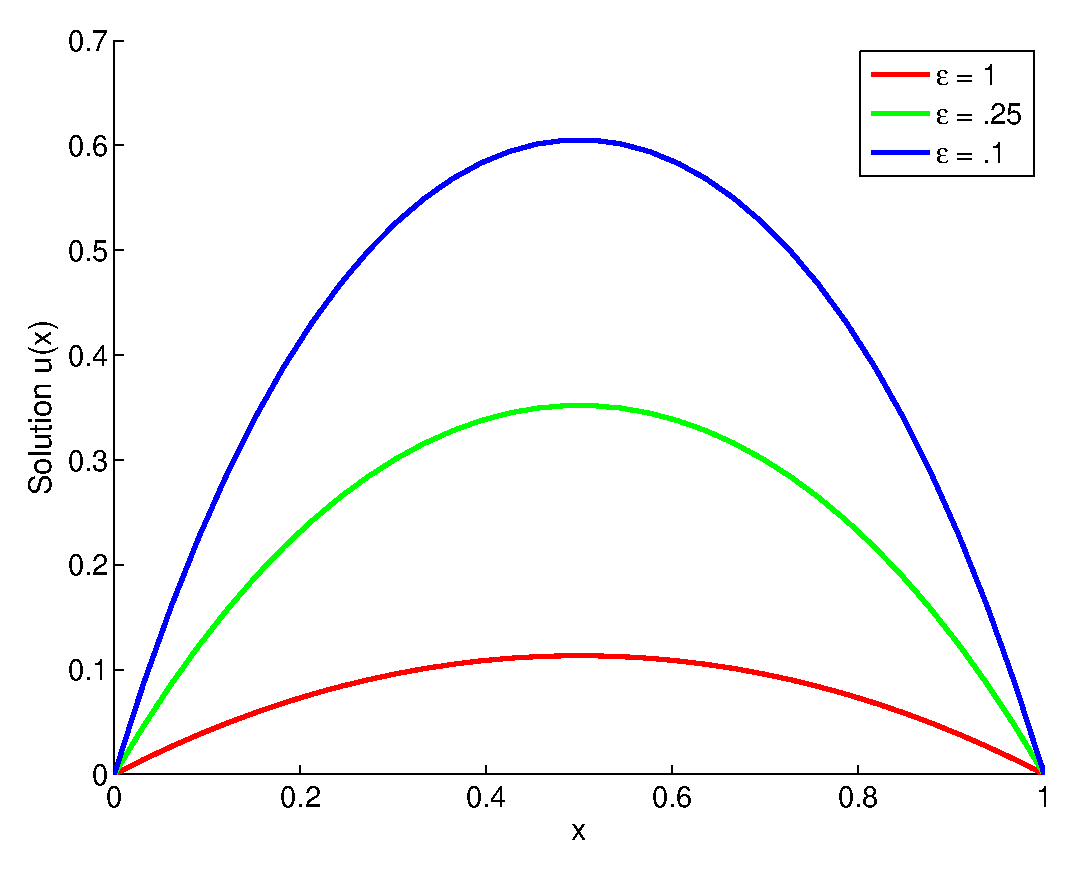
\includegraphics[width=0.42\textwidth]{ep1}\quad
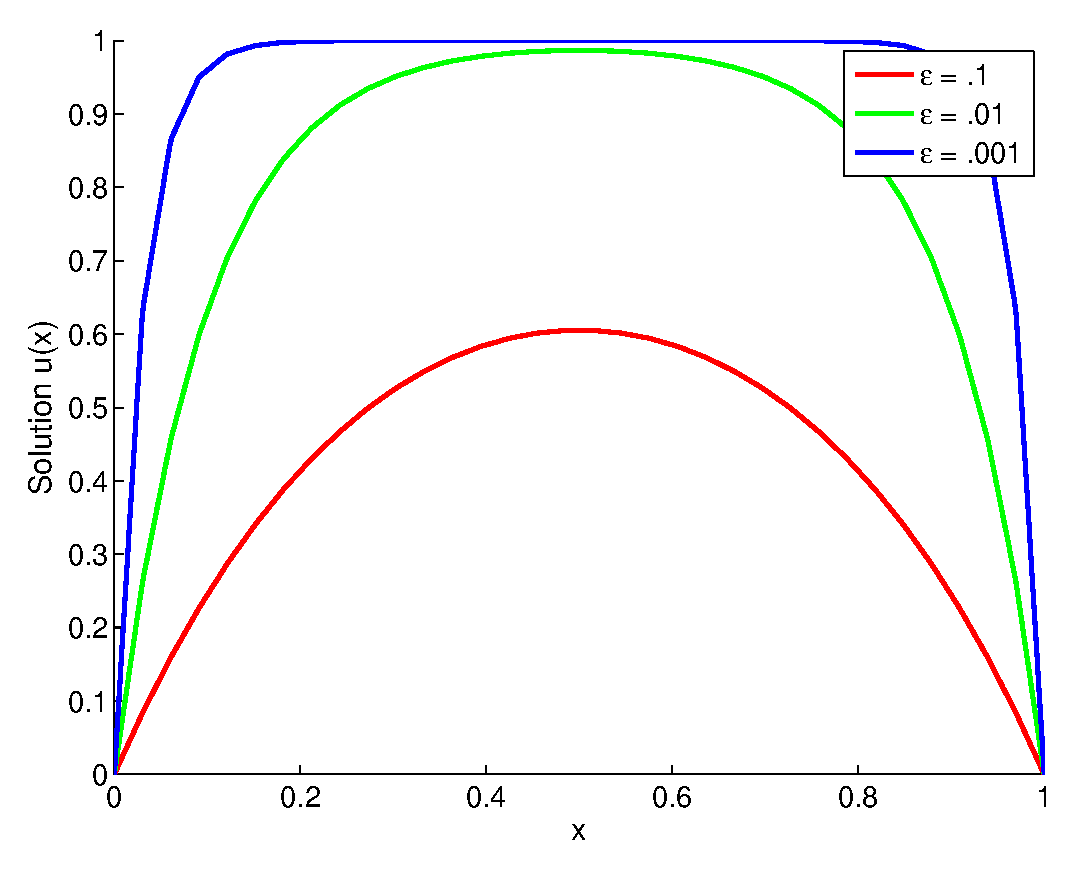
\includegraphics[width=0.42\textwidth]{ep2}
\end{center}

As $\epsilon$ decreases, the temperature in the bar increases.  It is difficult to see with $\epsilon \geq .1$, but as $\epsilon$ gets small, the solution actually develops additional characteristics called \emph{boundary layers}, where the solution becomes very steep near the boundaries.  \emph{Graders: please give credit just for noting the temperature increases, as the boundary layer phenomena was not visible for the range of $\epsilon$ specified in the problem.}

\item The process is very similar to part (a).  Multiply the differential equation with some function $v$
      from the space $V$ and integrate from $x=0$ to $x=1$ to obtain
     \[ \int_0^1 \bigg(-{d\over dx} \Big(k(x) {du \over dx}(x)\Big) v(x)
                      + p(x) u(x) v(x) \bigg)\,dx   
          = \int_0^1 f(x)v(x)\,dx.\]
      Break the integral on the left into pieces to obtain
     \[  \int_0^1 \bigg(-{d\over dx} \Big(k(x) {du \over dx}(x)\Big)\bigg) v(x)\,dx
       + \int_0^1 \bigg( p(x) u(x)\bigg) v(x)\,dx 
       = \int_0^1 f(x)v(x)\, dx.\]
     Integrate the first integral by parts to obtain
     \[ -\Big[ \kappa(x) {du \over dx}(x) v(x) \Big]_0^1 
        + \int_0^1 k(x) {du \over dx}(x) {dv\over dx}(x)\,dx
       + \int_0^1 \Big( p(x) u(x)\Big) v(x)\,dx 
       = \int_0^1 f(x)v(x)\, dx.\]
     The first term disappears because of the boundary conditions
     $v(0)=0$ and ${du(1)/dx} = 0$.  We consolidate the integrals
     on the left to arrive at the weak problem:
      \[ \mbox{Find $u\in V$ such that}\quad
          a(u,v) = (f,v) \quad \mbox{for all $v\in V$},\]
     where 
     \[ a(u,v) = 
         \int_0^1 \Big( k(x) {du \over dx}(x) {dv\over dx}(x)
                       + p(x) u(x) v(x)\Big)\,dx.\]
       
\item The proof for (e) is identical to the proof for (a).  \emph{Graders: please give full credit if the student notices this.}
\end{enumerate}
\end{solution}}{}

